\begin{surferIntroPage}{Primeiros passos}{tutorial_koord1}{Primeiros passos com o SURFER}
Este programa chama-se SURFER. Ao ler esta palavra, provavelmente ir\'a pensar em \'agua, sol e ondas. Mas neste caso a palavra vem de {\it surface} (palavra inglesa para superf\'icie).
\\
Com o SURFER podemos visualizar  superf\'icies, mais precisamente superf\'icies alg\'ebricas. O que isso significa e o que s\~ao superf\'icies alg\'ebricas, \'e explicado neste tutorial. Escolha uma das superf\'icies do lado direito para navegar atrav\'es dos cap\'itulos.\\
O SURFER faz parte da exposi\c c\~ao itinerante IMAGINARY, inaugurada durante 2008, o  Ano Alem\~ao da Matem\'atica. A exposi\c c\~ao \'e um projeto do internacionalmente conhecido Instituto de Investiga\c c\~ao Matem\' atica de Oberwolfach, na Alemanha. Neste instituto, todas as semanas se realizam  workshops sobre t\'opicos recentes na investiga\c c\~ao matem\'atica. Estes workshops s\~ao importantes para fomentar o interc\^ambio entre cientistas de todo o mundo. \\
\vspace{0.2cm} \hspace{3.5cm}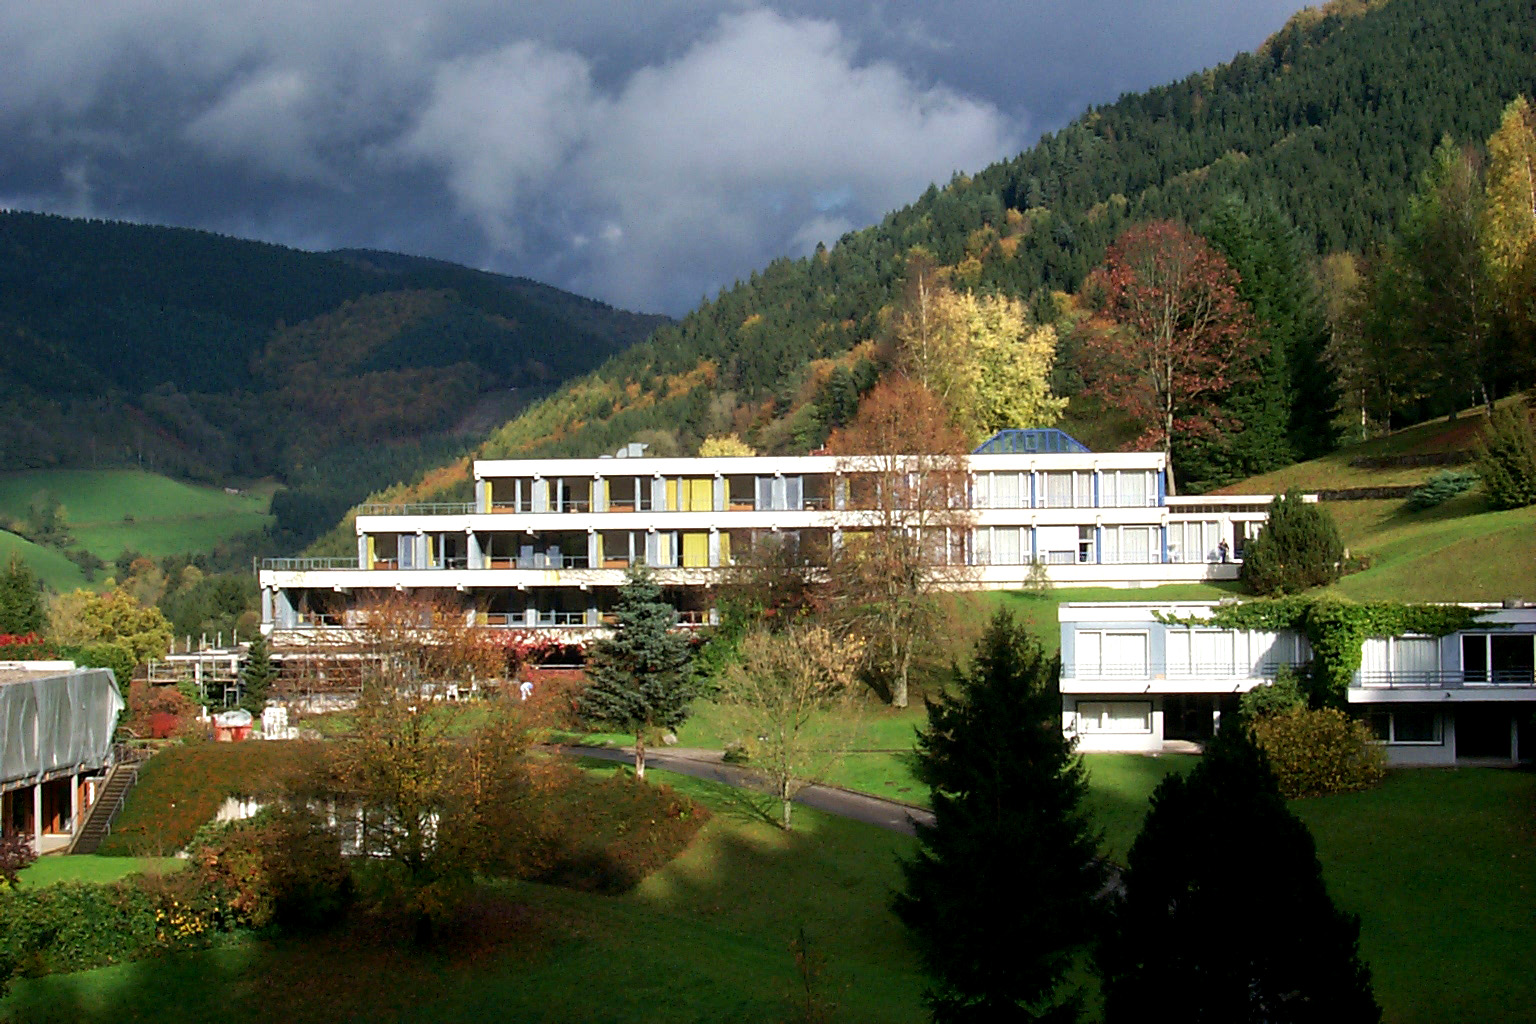
\includegraphics[width=3cm]{./../../common/images/photo_mfo.jpg}\\
O programa SURFER pode ser obtido gratuitamente atrav\'es do site: \\
\begin{centering}
www.imaginary-exhibition.com\\
\end{centering}
 \vspace{0.2cm}
\`A sua direita pode escolher um dos tutoriais matem\'aticos, a come\c car com a superf\'icie Citrus. \`A sua esquerda pode ir para outras galerias, por exemplo para a galeria  {\it Superf\'icies e Fantasia}.
\end{surferIntroPage}
